\title{Project 4: Neural Network Classifiers}
\author{Matthew R. Jenkins}
\date{\today}

\documentclass[12pt]{extarticle}
\usepackage[margin=1in]{geometry}
\usepackage{graphics}
\usepackage{graphicx}
\usepackage{float}
\graphicspath{{Figures/}}

\begin{document}
\maketitle

\section{Introduction}
This project focused on developing a neural network from scratch, and using testing data and varied layer structures to test its efficacy.

\section{Implementation}
My neural network used two classes - a NeuralNetwork class and a Node class. The Node class contains input and output values, as well as pointers to input nodes and output nodes. The input nodes just point to the nodes in the prior layer, whereas the output nodes contains pointers to nodes in the next layer, as well as weights for each node. The weighting is unidirectional because we can view a neural network as a directed graph, and there isn't much point in having the weights go in both directions for forward and back propagation.

The NeuralNetwork is simply a class which contains 3 lists: an input layer, a hidden layer, and an output layer. The hidden layer is a two dimensional list, which allows it to have more than one hidden layer inside of it. Each list has a bunch of nodes inside of it, and those are connected to using the input and output nodes above.

Aside from that, back-propagation and other algorithms such as k-fold cross validation were simple(ish) to implement. Some challenges arose, such as getting the previous input's output weights, but I was able to get the algorithms given to behave. One thing I wish I could've done was make the code more laconic - I feel like a lot of my code was redundant and could be better optimized.

\section{Results}
To gather results, I decided to analyze possible hidden layer permutations and their accuracy. To do this, I wrote a test automation function, \verb$testing_nn_layout$, which takes a data set, data set name (for file I/O), a default input layer size, and a default output layer size. These are done to garner the efficacy of different Neural Network structures. 

I decided to focus more on the structure of the neural networks rather than every specific minute detail, such as a decaying alpha or whether the Neural Network would work with multi-class problems. This was done to simplify my results gathering a little bit. I decided to do so by making one to two differently sized hidden layers, with 1 to 8 hidden nodes inside each. 

The only controls (elements which I needed to keep consistent) I found were the number of epochs - which I kept as 1000 for testing purposes, as well as the alpha (which I kept as $1000 / 1000 + t$, where t is the number of epochs). Aside from that, everything was dependent on size of the inputs as well as the number of examples.

The binary classification data-sets used for analysis are as follows:
\begin{itemize}
  \item \verb$generated.csv$. This contains three points per example: 2 x points, and 1 y point (0 or 1). There are 100 examples in this set. This is a simple x-y plot, with class easily separable by a line.
  \item \verb$breast-cancer-wisconsin-normalized.csv$. This contains 30 x points, and 1 y point (0 or 1) per example. There are 570 examples in this set. This is named as such because the data is used to "teach" neural networks how to detect if a person is at risk for breast cancer.
  \item \verb$banana.csv$. This contains three points per example: 2 x points, and 1 y point (0 or 1). There are about 5300 examples in this set. This is named banana due to classified data points in one class being shaped like an upside down banana. This is a more complex problem compared to the prior two.
\end{itemize}

In order for our neural networks to be effective, they need to produce results greater than perceptrons, given the same problem. Perceptrons are simply neural networks which do not contain hidden layers. Perceptrons solving the above data-sets resulted in the following percentages (rounded to 1 decimal place):
\begin{itemize} 
\item \verb$generated.csv$: $92.0\%$
\item \verb$breast-cancer-wisconsin-normalized.csv$: $95.1\%$
\item \verb$banana.csv$: $44.8\%$
\end{itemize}

These results were gathered by running the \verb$linear_classifier.py$ on the data-sets mentioned above.

The sets of data were split into two subcategories - neural networks with 1 hidden layer (with nodes from 1 to 8), and neural networks with 2 hidden layers (hidden layer 1 staying consistent but having nodes in the range from 1 to 8, and hidden layer 2 containing nodes from 1 to 8). Testing these takes exponential time depending on how many layers there are, so I capped it at 2 hidden layers with 8 nodes each to make testing brief.

\subsection{One-dimensional hidden layers}

\begin{figure}[H]
\centering
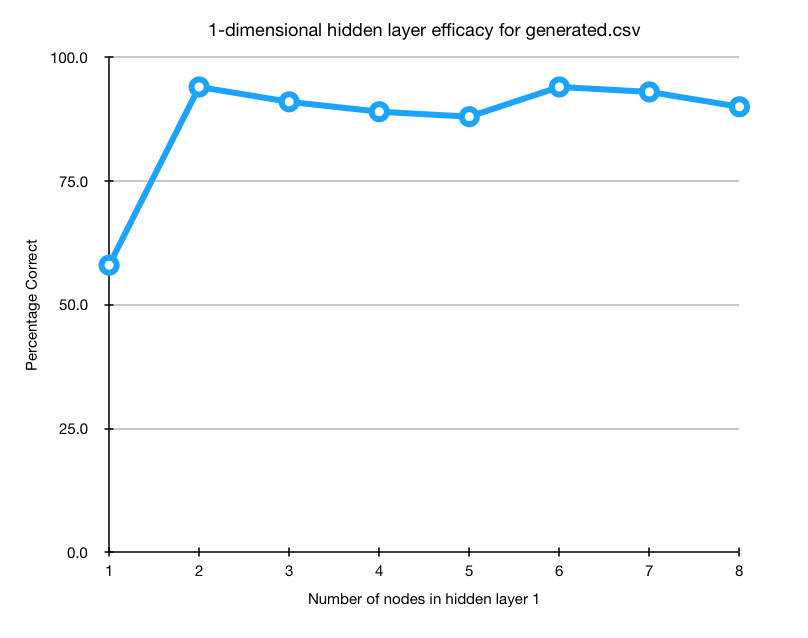
\includegraphics[width=0.6\linewidth]{generated-1d}
\end{figure}

Quite a few data-points were able to produce greater accuracy than our linear classifier (more specifically a hidden layer with nodes 2, 6, and 7 produced a greater accuracy than our default 92.0\%).

\begin{figure}[H]
\centering
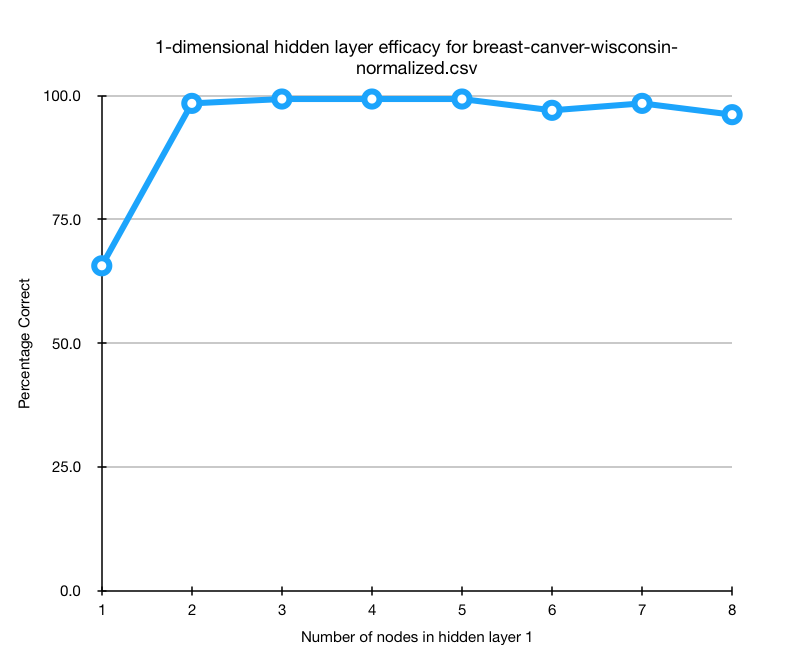
\includegraphics[width=0.6\linewidth]{breast-1d}
\end{figure}

Pretty much any neural network with a node count greater than 2 produced greater results than our classifier (all were greater than or equal to 95.1\%). Note: the misspelling of cancer was an oversight.

\begin{figure}[H]
\centering
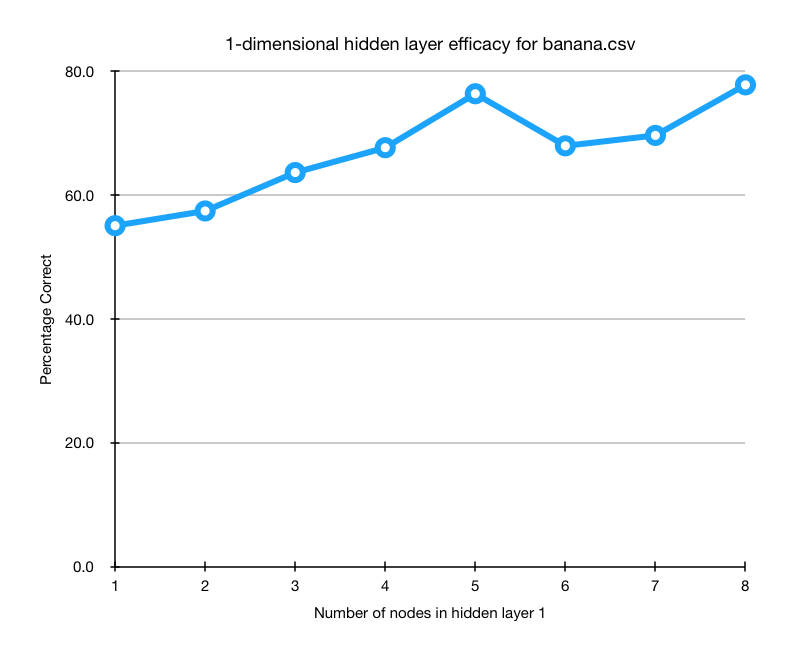
\includegraphics[width=0.6\linewidth]{banana-1d}
\end{figure}

Note the upper bound value is different than the other two graphs. While all the data-points have higher accuracy than the linear classifier (for reference: 44.8\%), it's still rather disappointing to see the lack of performance of this in comparison to the other two examples. But again, this is a more complex problem than the other two.

\subsection{Two-dimensional hidden layers}

\begin{figure}[H]
\centering
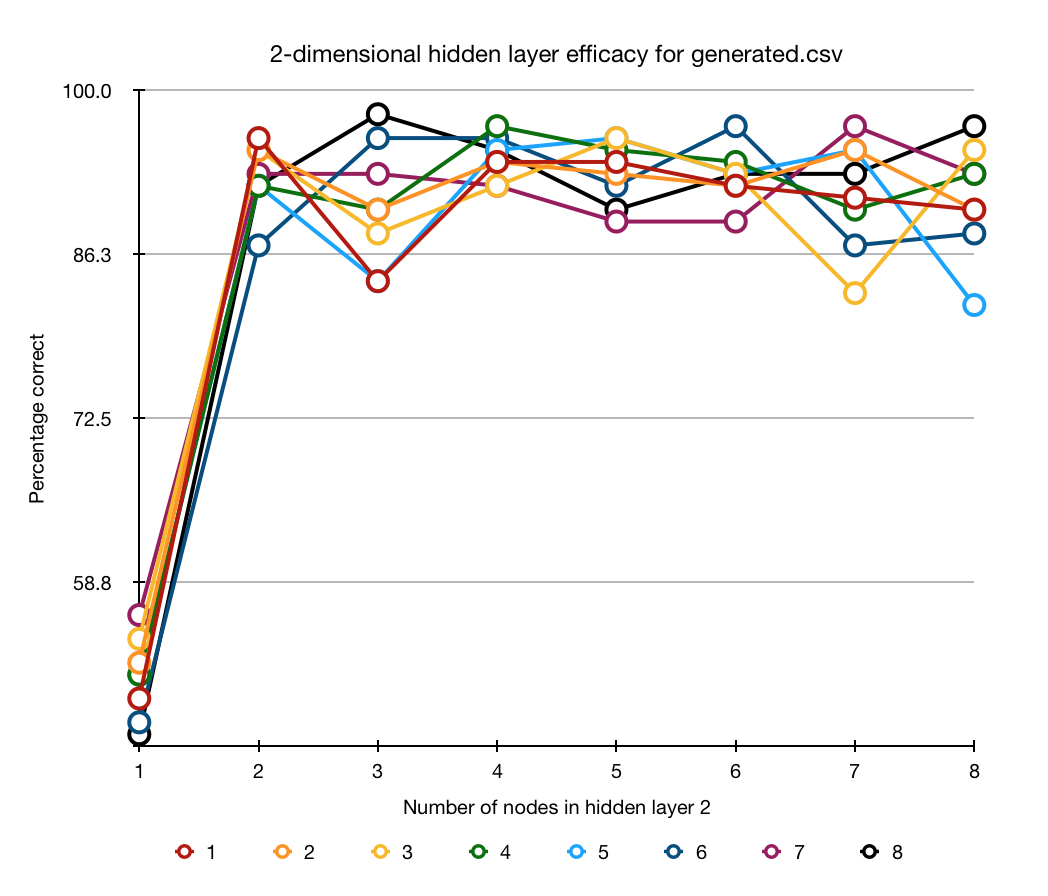
\includegraphics[width=0.6\linewidth]{generated-2d}
\end{figure}

The average of each line results in a steady increase in accuracy over time, but this is best seen with the hidden layer 8 nodes, as it has 5 different node amounts which produces a greater accuracy than the linear classifier (92.0\%).

\begin{figure}[H]
\centering
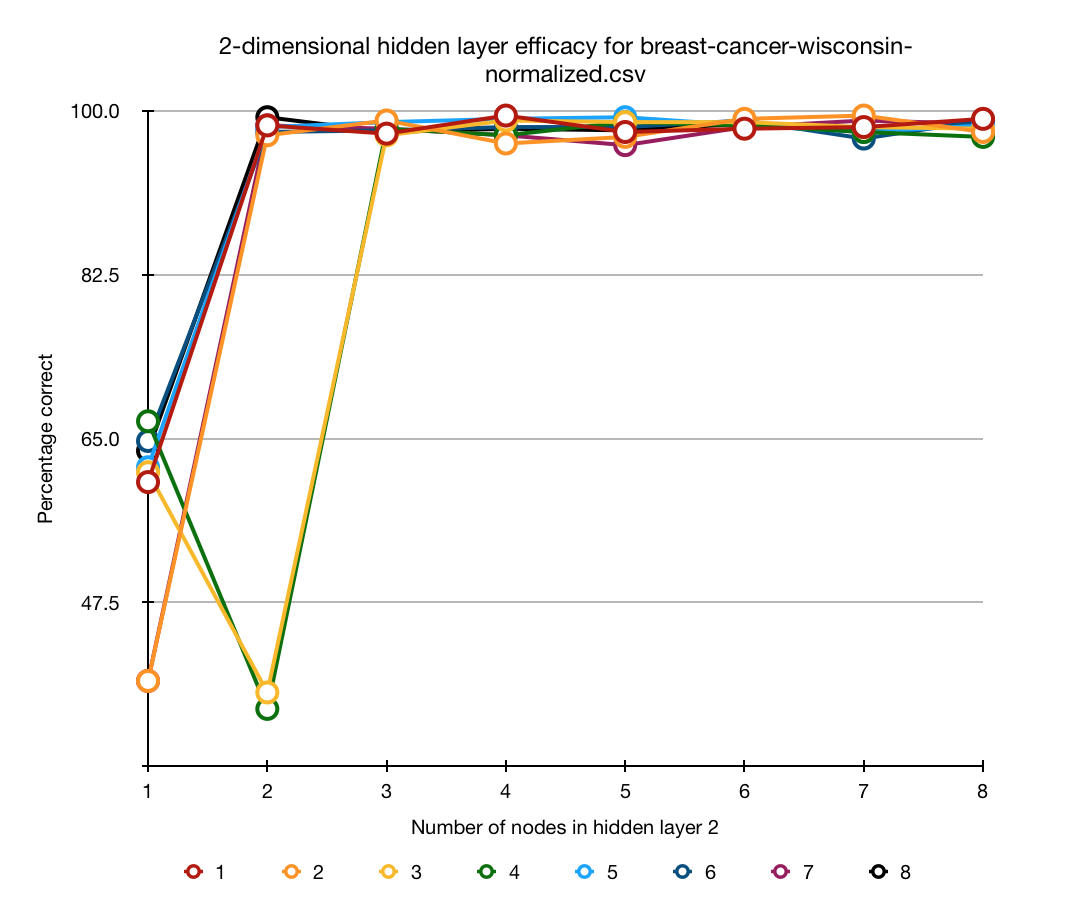
\includegraphics[width=0.6\linewidth]{breast-2d}
\end{figure}

Similar to the 1-dimensional, nearly all of them pass with flying colors and do greater than the linear classifier (95.0\%). I'm personally surprised 3 and 4 had a delay in reaching the asymptote compared to the others - I'm not sure what to chalk that up to.

\begin{figure}[H]
\centering
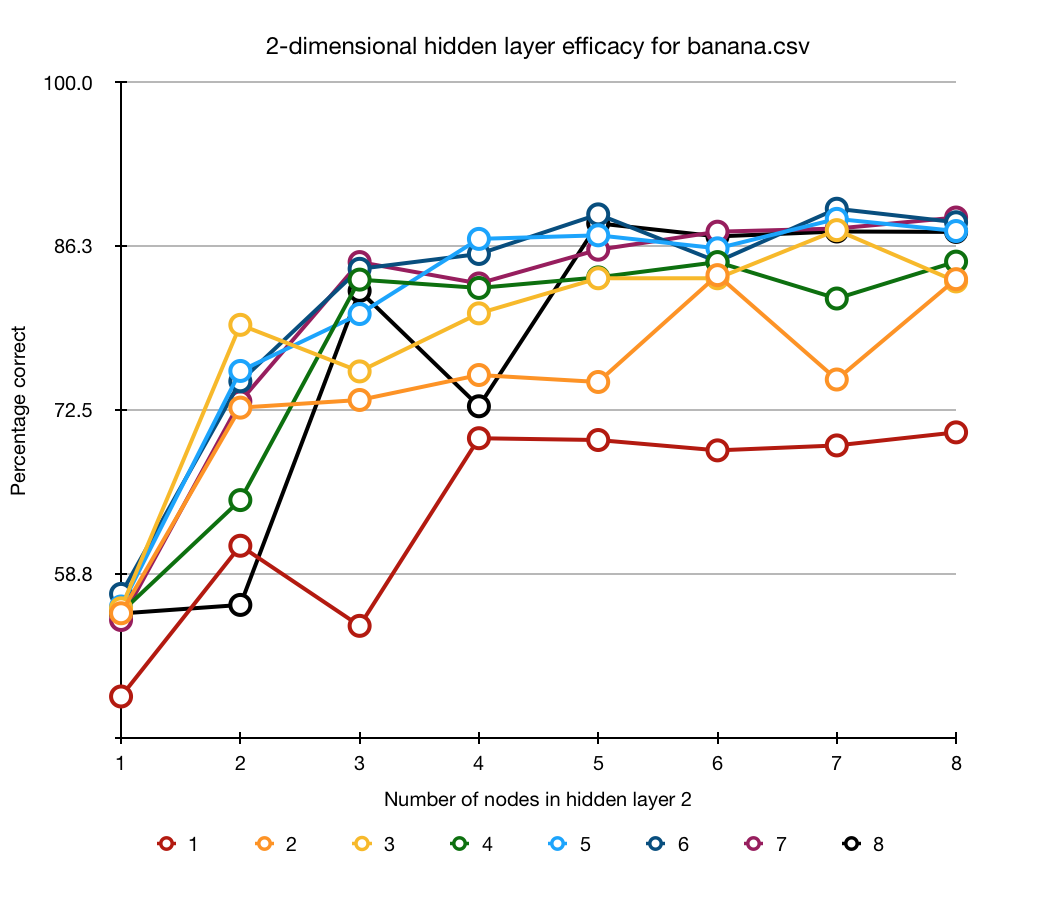
\includegraphics[width=0.6\linewidth]{banana-2d}
\end{figure}

In this case, there is a noticeable trend of higher hidden layer node amounts doing better at this classification problem than others. This makes sense, as this is much less clear-cut of a classification problem than the other two. Despite the low-ish numbers, all values are still greater than our linear classifier (44.8\%).

Doing an average of the data leads to the conclusion that 6 nodes solves this problem best.

\section{Discussion}

Some observations I've noticed are that singular neural networks kind of sucked (to put it nicely), the sweet spot seemed to be between 2-7 nodes for most linear classification problems, and for more complex problems, more nodes provide better accuracy.

I feel that single node neural nets weren't the best because it was doing linear classification implicitly into the single hidden layer. The hidden layer didn't really do much other than pass that result to the output with slight modifications, so whatever result was produced was just pushed out. More nodes (understandably) allowed for more computation of the inputs, and thus better accuracy.

The sweet spot of my testing seemed to be between 2 and 7 nodes for most linear classification problems. As mentioned in class, neural networks are used in cases where classifying things based on input isn't so concrete. By using a neural network in lieu of something simple we're really throwing computational power at the wall at a specific point. In more complex classification cases, we're not exactly throwing computational power at the wall, as more nodes tends to provide better and better results for them. Perhaps the true use case of neural networks is when we can throw time and computational power at a problem. We just want results, in most cases - optimization can be a secondary factor.

This being said, my studies have had limitations. I omitted multi-class data-sets due to time concerns. I also didn't use data-sets aside from the ones provided, mostly because I thought the data-sets provided would be a good microcosm of examples, though I am realizing now there could be possible over-fitting of data with them. I also felt like I could have used more varied numerical analysis in the results section instead of capping it at a somewhat small power of two, but again, this was done due to time concerns.

% observations:
% single node neural nets kinda sucked, worse than a linear classification problem - any specific reasons why?
% sweet spot seemed to be between 2 and 7 nodes for most linear classification problems, though this led to some diminishing returns.
% for more complex problems such as the banana dataset, more nodes provided better results.

% limitations:
% lack of multi-class data-sets
% lack of usage of non-provided data-sets
% more hidden layer size analysis?

\end{document}